\documentclass[tikz,border=2mm]{standalone}
\usetikzlibrary{matrix,backgrounds}

\begin{document}
	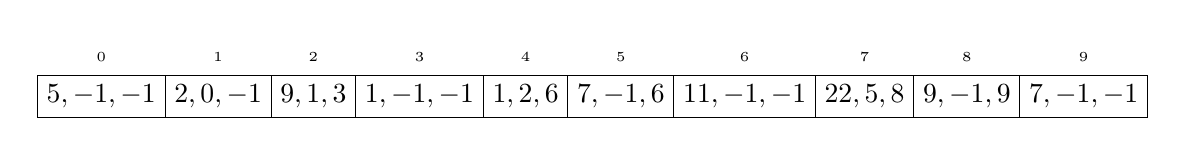
\begin{tikzpicture} [nodes in empty cells,
	nodes={minimum width=0.5cm, minimum height=0.5cm},
	row sep=-\pgflinewidth, column sep=-\pgflinewidth]
	border/.style={draw}
	
	\matrix(vector)[matrix of nodes,
	row 1/.style={nodes={draw=none, minimum width=0.3cm}},
	nodes={draw}]
	{
		\tiny{0} & \tiny{1} & \tiny{2} & \tiny{3} & \tiny{4} & \tiny{5} & \tiny{6} & \tiny{7} & \tiny{8} & \tiny{9} \\
		$5, -1, -1$ & $2, 0, -1$ & $9, 1, 3$ & $1, -1, -1$ & $1, 2, 6$ & $7, -1, 6$ & $11, -1, -1$ & $22, 5, 8$ & $9, -1, 9$ & $7, -1, -1$ \\
	};
	\end{tikzpicture}
\end{document}